\documentclass[12pt]{article} % die ersten vier Packages sind immer Pflicht
\usepackage[utf8]{inputenc}
\usepackage[ngerman]{babel}
\usepackage[T1]{fontenc}
\usepackage{helvet} % andere Schriftarten 
\usepackage[margin=3cm]{geometry} % Seitenrand auf 3cm
\usepackage{setspace} % ermoeglicht Abstandsaenderung s.u.
\usepackage{graphicx} % Import von Abbildungen
\usepackage{apacite} % wichtig fuers zitieren
\usepackage{natbib} % wichtig fuers zitieren
\usepackage{titling} % Anpassen der Titel
\usepackage[hidelinks]{hyperref} % verlinkt alle Zitate und das toc
\usepackage[usenames,dvipsnames]{color}    
\usepackage{tocloft} % sorgt fuer ein numeriertes Literaturverzeichnis
\usepackage{caption} % macht Tabellen und Abbilungsbeschreibung
\DeclareCaptionLabelSeparator*{spaced}{\\[1.2ex]} % veraendert mit nachfolgenden Befehlen die Tabellen und Abbildungsbeschreibung nach APA
\captionsetup[table]{textfont=it,format=plain,justification=justified,
	singlelinecheck=false,labelsep=spaced,skip=2pt}
\captionsetup[figure]{labelsep=period,labelfont=it,justification=justified,
	singlelinecheck=false}
\usepackage{titlesec} % anpassen der groesse der ueberschriften
\usepackage{array,multirow} % fortgeschrittene Graphen und Tabelleneinteilung
\usepackage[nottoc,numbib]{tocbibind} % fuers Inhaltsverzeichnis
\usepackage{amsmath} % diverse mathematischen Dinge, aber auch die Moeglichkeit mit \text{} Text zu gruppieren. Hilfreich, wenn LaTeX bei 3 000 bspw. die 3 in die obere und die 000 in die unteren Zeile schreibt
\usepackage{listings}

\titleformat*{\section}{\Large\bfseries} % greift auf Package titlesec zurueck
\titleformat*{\subsection}{\large\bfseries}
\titleformat*{\subsubsection}{\normalsize\bfseries}

\graphicspath{ {images/} } % setzt Abbildungspfad auf einen Ordner namens "images" innerhalb des Verzeichnisses, in dem dein .tex File liegt
\renewcommand{\familydefault}{\sfdefault} % aendert die schriftart
\renewcommand{\baselinestretch}{1.5} % 1.5 facher Zeilenabstand
\renewcommand{\cftsecleader}{\cftdotfill{\cftdotsep}} % macht im Inhaltsverzeichnis Punkte auch bei Hauptueberschriften
\renewcommand{\arraystretch}{1.1} % veraendert den Abstand zwischen Tabellenzellen

\title{Bachelorarbeit} % eigentlich ueberfluessig, wenn kein Deckblatt mit \maketitle gewuenscht
\author{Jan Philipp Nolte}
\date{01. Mai 2018}

\begin{document}
	
	\lstset{ % veraendert den Stil der R Syntax. Wenn kein R Code integriert, einfach komplett loeschen
		language=R,                     % the language of the code
		basicstyle=\small\ttfamily, % the size of the fonts that are used for the code
		numbers=left,                   % where to put the line-numbers
		numberstyle=\small\color{Blue},  % the style that is used for the line-numbers
		stepnumber=1,                   % the step between two line-numbers. If it is 1, each line % will be numbered
		numbersep=5pt,                  % how far the line-numbers are from the code
		backgroundcolor=\color{white},  % choose the background color. You must add \usepackage{color}
		showspaces=false,               % show spaces adding particular underscores
		showstringspaces=false,         % underline spaces within strings
		showtabs=false,                 % show tabs within strings adding particular underscores
		frame=single,                   % adds a frame around the code
		rulecolor=\color{black},        % if not set, the frame-color may be changed on line-breaks within not-black text (e.g. commens (green here))
		tabsize=2,                      % sets default tabsize to 2 spaces
		captionpos=b,                   % sets the caption-position to bottom
		breaklines=true,                % sets automatic line breaking
		breakatwhitespace=false,        % sets if automatic breaks should only happen at whitespace
		keywordstyle=\color{RoyalBlue},      % keyword style
		commentstyle=\color{ForestGreen},   % comment style
		stringstyle=\color{ForestGreen}      % string literal style
	}
	
	\pagenumbering{Roman} % veraendert die Art der Seitennummerierung
	
	\tableofcontents 	

	\newpage
	
\section*{Zusammenfassung}
	
	\citet{draxler2015power} haben eine Klasse pseudo-exakter oder konditionaler Tests zur Power-Berechnung von Annahmen des Rasch Modells vorgeschlagen. Zum Simulieren der für die Power-Berechnung notwendigen Daten bedarf es Sampling-Algorithmen. \citet{verhelst2008efficient} hat mit dem \textit{Rasch Sampler} einen relativ schnellen Algorithmus entworfen, der die wahre Verteilung mithilfe von \textit{Markov Chain Monte Carlo} Prozeduren approximiert. \citet{miller2013exact} haben mit dem \textit{Exact Sampler} einen Algorithmus entwickelt, der die exakte Verteilung abzählen und daraus ziehen kann. Die Genauigkeit der beiden Sampler wird verglichen, indem potentielle Einflüsse der Stichprobengröße, DIF-Parameter und Itemschwierigkeit auf die Genauigkeit der Power-Berechnung untersucht werden. Darüber hinaus werden die Burn-In Phase und der Step-Parameter als Einflussfaktoren auf den \textit{Rasch Sampler} überprüft. Die Genauigkeit der Sampler unterscheidet sich nicht wesentlich. Bei steigender Stichprobengröße steigt die Power an. Auch bei größeren Modellabweichung im Positiven wie im Negativen kann eine höhere Power beobachtet werden. Bei moderater Itemschwierigkeit ist die Power bei positivem und negativem DIF-Parameter nahezu gleich groß und bei Modellabweichung eines leichten Items ist die Power bei positiver Abweichung größer als bei negativer. Mit einem schwierigen Item ist mit dem Unterschied, dass die Streuung deutlich höher ausfällt, ein gegensätzlicher Trend zu beobachten. Weder die Burn-In Phase noch der Step-Parameter hat einen Einfluss auf die Genauigkeit des \textit{Rasch Samplers}. Aufgrund von effizienterer Berechnung sollte in jedem Fall der \textit{Rasch Sampler} verwendet werden.	Die Ergebnisse bezüglich des Verhaltens der Power unter Variation verschiedener Parameter entsprechen den Beobachtungen von \citet{draxler2015power}. 	
	\begin{flushleft}
		\textbf{Schlüsselwörter:} Rasch Modell, Power, Pseudo-exakte Tests, Konditionale Tests, Rasch Sampler, Exact Sampler	
	\end{flushleft}
	
	\newpage
	\pagenumbering{arabic}
	
\section{Einleitung}
	
	Die psychologische Testtheorie ist in der Psychologie eine der Grundlagen für neue Erkenntnisse. Anders als zum Beispiel bei der Körpergröße, sind viele interessierende Dimensionen in der Psychologie nicht direkt messbar. Derartige Merkmale nennt man latent. Jedes Mal, wenn ein latentes Merkmal sichtbar gemacht werden soll, muss man einen psychologischen Test anwenden. Dabei können die Anwendungsbereiche von Intelligenzquotienten über Persönlichkeitsmerkmale bis hin zur Erfassung ganzheitlicher Arbeitsbedingungen alle nur erdenklichen Bereiche der Psychologie abdecken. Aber auch in anderen Fachbereichen finden testtheoretische Ansätze Anwendung. Es gibt grundsätzlich zwei Ansätze: die klassische und die probabilistische Testtheorie. Für diese Arbeit ist ausschließlich Letztere von Bedeutung. Die probabilistische Testtheorie geht davon aus, dass die Ausprägung des gemessenen Merkmals sowohl von der Personenfähigkeit als auch von der Itemschwierigkeit abhängt. Dabei gibt es je nach Anwendungsbezug im Rahmen der \textit{Item response theory} (IRT) Modelle, mithilfe man die Wahrscheinlichkeit ausrechnen kann, einen bestimmten Wert für ein bestimmtes Item zu erzielen. Bei einer erneuten Testung der Personen würde die Wahrscheinlichkeit für eine Antwort $x$ gleich bleiben, aber das Ergebnis könnte variieren, da der Zusammenhang nicht deterministisch festgelegt ist. Die probabilistische Testtheorie hat in den letzten Jahren vermehrt an Bedeutung gewonnen, was weniger an der kürzlichen Erschließung des theoretischen Fundaments, sondern viel mehr an dem rasanten Fortschritt der Technik liegt, die es benötigt, um Kalkulationen unter der IRT durchzuführen. Ein bekanntes Anwendungsbeispiel sind die PISA-Studien \citep*{prenzel2007pisa}. Da die Lernpläne zwischen den verschiedenen Ländern nicht identisch sind, können nur IRT Modelle einen adäquaten Vergleich schaffen.
	
	Eine zentrale Größe vor und nach der Durchführung eines Tests ist die Anzahl der richtigen und falschen Ergebnisse. Wie oft erkennt der Test zum Beispiel eine pathologische Diagnose, obwohl der Patient gesund ist und wie oft wird der Patient gesund eingeschätzt, obwohl dieser eine Erkrankung hat? Während ersterer Frage in der Vergangenheit bereits viel Aufmerksamkeit zuteil wurde, hat man die Wichtigkeit letzterer länger unterschätzt. Dabei kann dieser Fehler je nach Kontext nicht nur genauso relevant sein wie der erste, sondern noch tiefgreifender. Angenommen, ein Test soll Schizophrenie diagnostizieren. Nach der Diagnose erhält der Patient ein starkes Neuroleptikum mit schwerwiegenden Nebenwirkungen. Der erste Fehler beschreibt die Wahrscheinlichkeit, dass ein Patient, der keine Schizophrenie hat, das Neuroleptikum verschrieben bekommt. Das ist sicherlich nicht erwünscht, aber der zweite Fehler beschreibt in diesem Fall die Wahrscheinlichkeit, dass eine schizophrene Person als gesund diagnostiziert und unbehandelt nach Hause geschickt wird. Diese letztere Wahrscheinlichkeit kann kontrolliert werden. Man sollte die Power -- die Gegenwahrscheinlichkeit besagten Fehlers -- eines statistischen Tests, wie \citet{draxler2010sample} vorgeschlagen hat, genau wie den Fehler erster Art a priori festlegen und aufgrund dessen die für eine gewünschte Genauigkeit benötigte Stichprobengröße ausrechnen. 
	
	Im Anwendungskontext von Modellen unter der IRT kann die Power mithilfe von Simulationen berechnet werden. Für diese Simulationen gibt es zwei verschiedene Ansätze. Einerseits ein relativ schnelles, approximatives Verfahren und andererseits ein langsameres Verfahren, bei dem die exakte Verteilung bekannt ist. Da der exakte Algorithmus extrem rechenintensiv ist, muss die Frage gestellt werden, in welchen Szenarien es genügt, die zugrunde liegende Verteilung zu approximieren und wann oder ob überhaupt die Notwendigkeit der exakten Berechnung besteht. Auch ist es durch die exakte Funktion zum ersten Mal möglich, die Genauigkeit des approximativen Verfahrens im Allgemeinen zu überprüfen, da die genaue Verteilung bekannt ist. Diesen Fragen sowie dem Abklären potentieller Einflüsse verschiedener Parameter auf die Power-Berechnung evaluiert diese Arbeit.
	
\subsection{Theoretischer Hintergrund}

	Im Folgenden werden die für diese Arbeit notwendigen theoretischen Fundamente vom binären Rasch Modell über die Berechnung der Power pseudo-exakter oder konditionaler Tests von Annahmen des Modells nach Draxler und Zessin (2015) bis hin zum Vergleich der Funktionsweise verschiedener Sampling-Algorithmen erklärt. 
		
\section{Methodik}
	Im Folgenden wird das genaue Studiendesign zur Beantwortung der sechs Fragestellungen und die für die Datenanalyse verwendete Hardware und Software vorgestellt. 

\subsection{Studiendesign}
	Für sämtliche Berechnungen wird $\alpha$ mit 5 Prozent gewählt. Die Anzahl der gezogenen Matrizen wird bei Fragestellung A auf 3 000 und bei Fragestellung B bis E auf 8 000 festgesetzt, da diese als genügend groß angenommen werden kann, um die gesamte Verteilung abzubilden ...

\section{Ergebnisse}
[...]
Auffällig ist die bedeutend höhere Standardabweichung bei 150 Personen und 4 Items. Diese ist mit \text{\textit{SD} = 0.063} beim \textit{Rasch Sampler} und \text{\textit{SD} = 0.064} beim \textit{Exact Sampler} mit der Ausnahme von 60 Personen, da dort einige Ausreißer zu beobachten sind, bedeutend höher als bei anderen Personenkonstellationen, die in einem Bereich von 0.009 und 0.026 liegen. Des Weiteren ist die Power bei beiden Samplern bei der 30 x 4 Matrix mit \textit{M} = .25 und \textit{SD} = 0.014 respektive \textit{M} = .25 und \textit{SD} = 0.013 beim \textit{Exact Sampler} deutlich niedriger als die der anderen Matrizen. An diesen Beispielen kann man exemplarisch auch erkennen, wie gering die Unterschiede zwischen den Samplern sind. Die Matrix mit zehn Personen weist mit \textit{M} = .59 die größte mittlere Power auf. Auffällig ist außerdem die fehlende Kontinuität beider Sampler. Bei steigender Personenzahl ist kein linearer Zusammenhang in Form von steigender Power beobachtbar. In Abbildung \ref{fig:samplesize} wird der in Fragestellung B untersuchte Zusammenhang zwischen der Power und der Stichprobengröße illustriert. 
\begin{figure}[ht]
	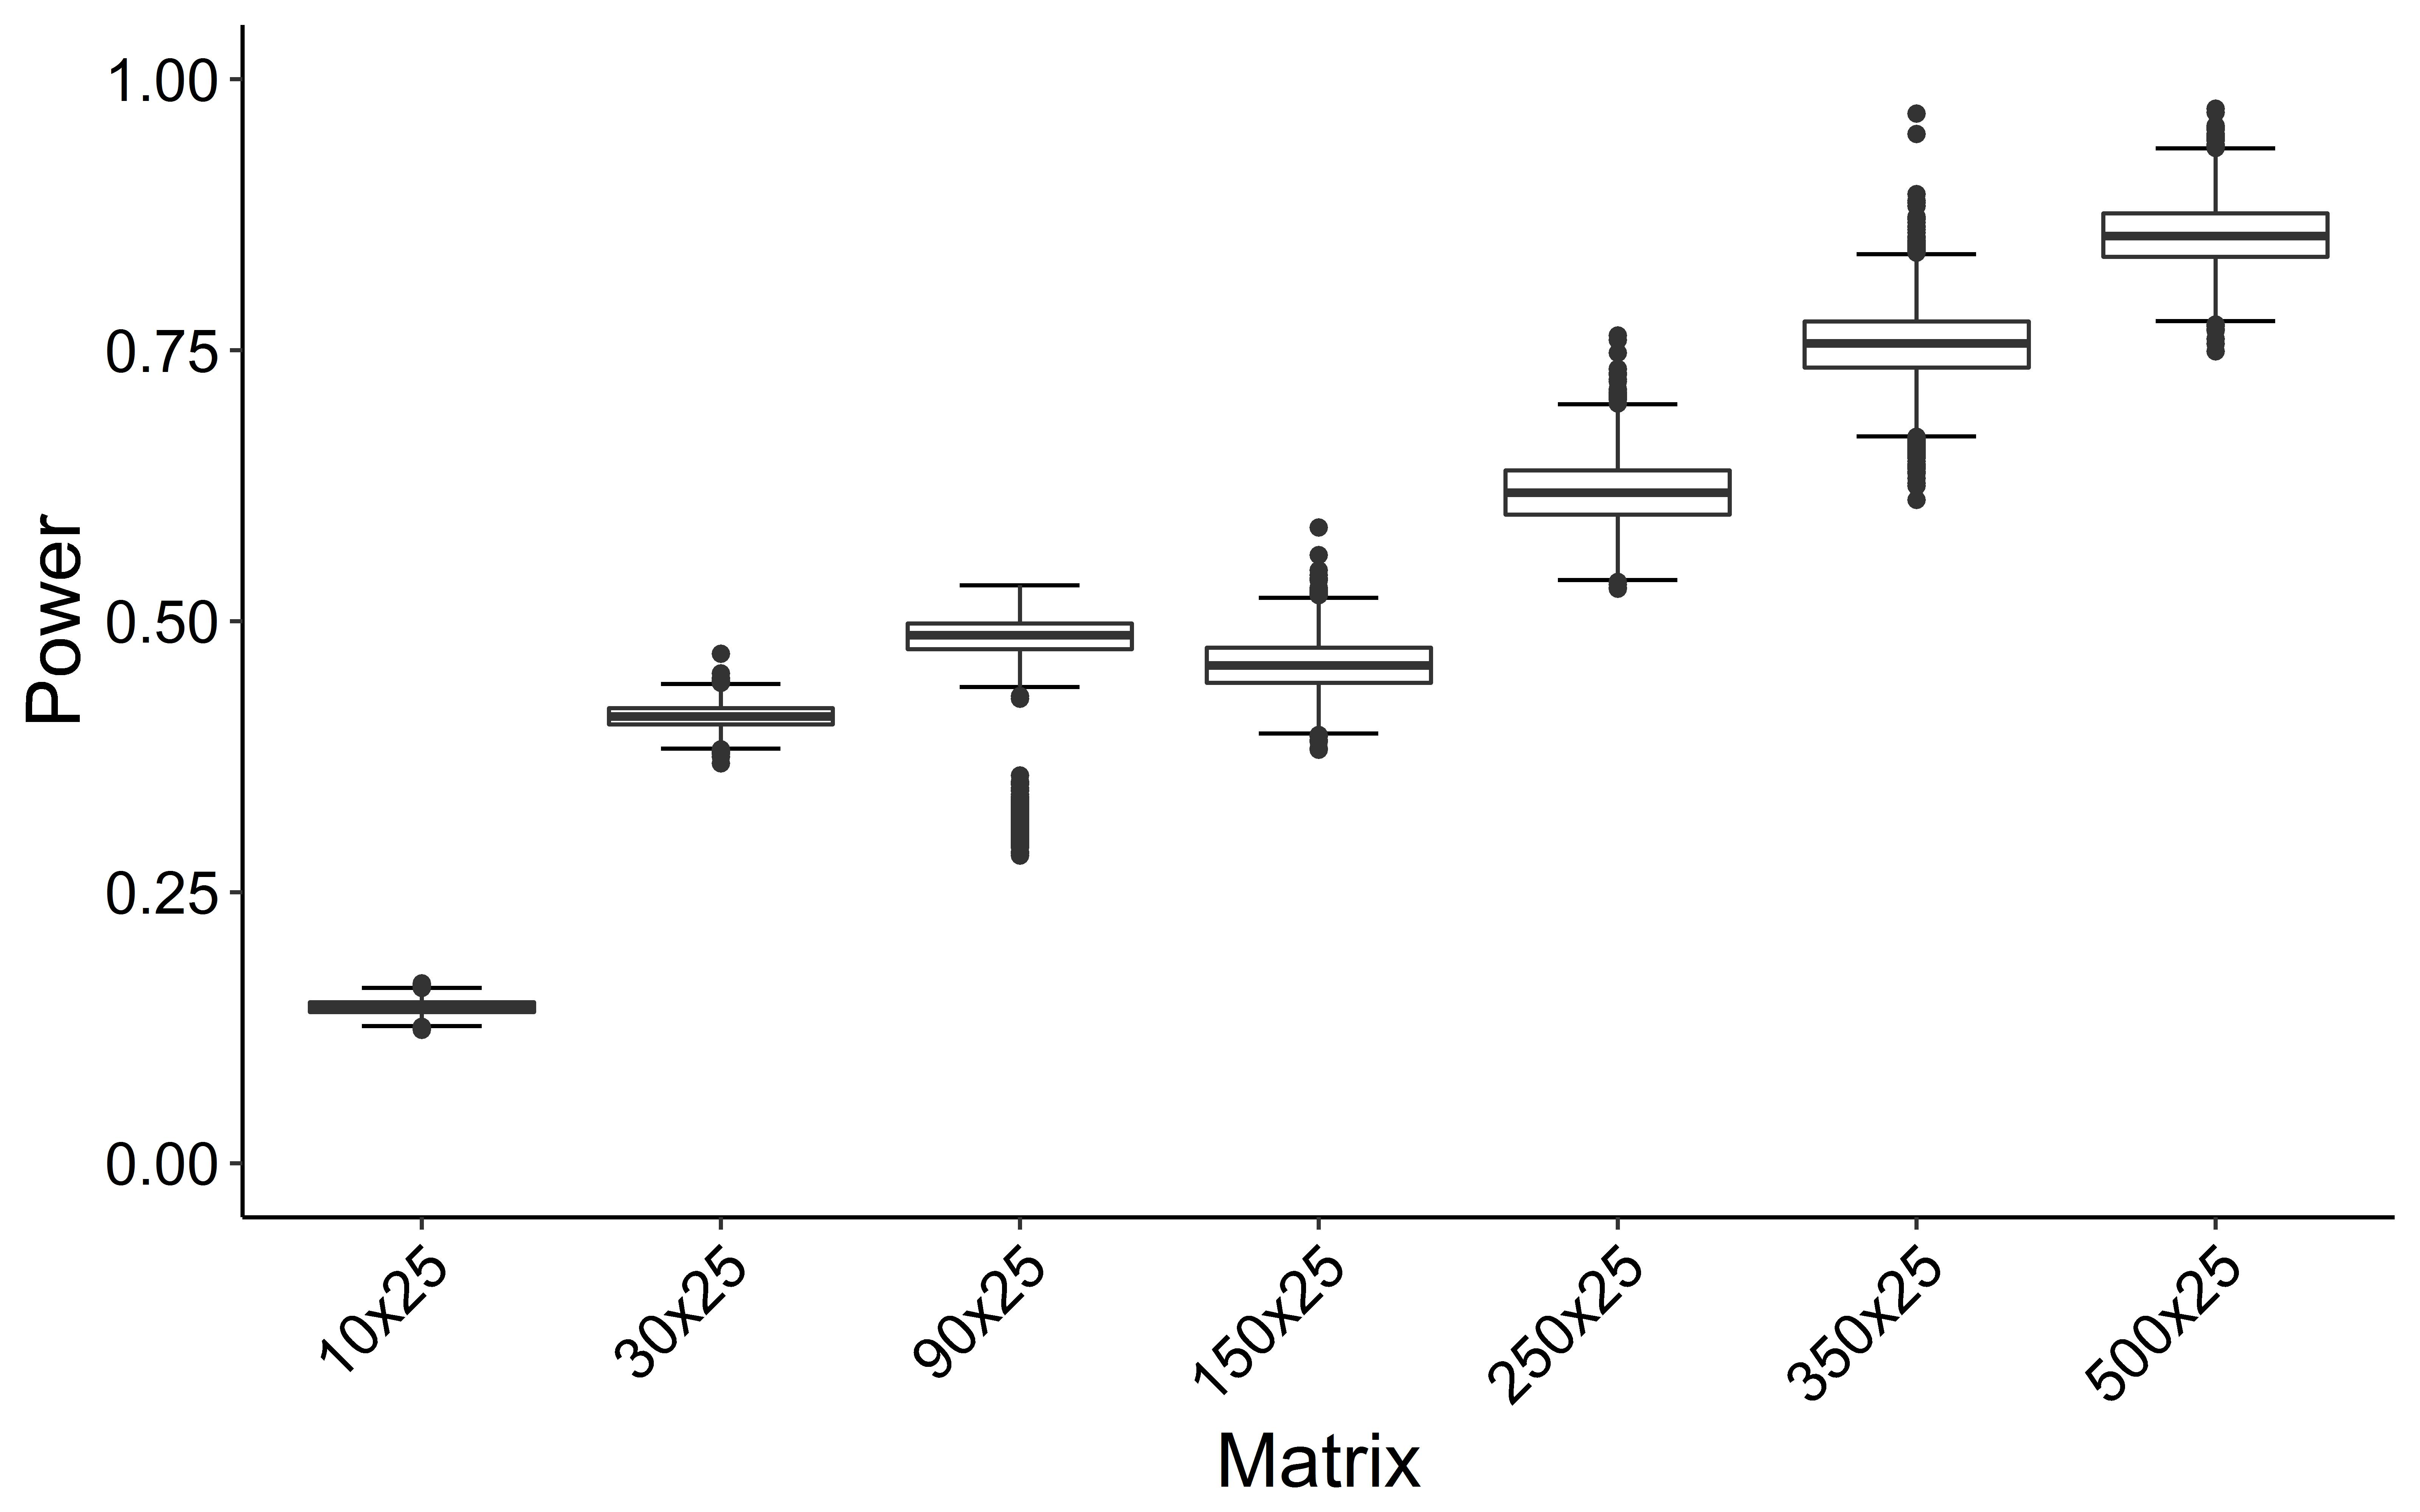
\includegraphics[width=0.79\textwidth]{B.jpeg}
	\caption{Box Plots der Wahrscheinlichkeitsverteilung der Power verschiedener Stichprobengrößen bei gleichbleibender Itemanzahl}
	\label{fig:samplesize}
\end{figure}
[...]
\begin{table}[ht]
	\caption{Deskriptive Statistik zu Abbildung \ref{fig:samplesize} mit Minimum (Min), 2.5\% Quantil (Q.025), 25\% Quantile (Q.25), Median, Mittelwert (Mean), 75\% Quantil (Q.75), 97.5\% Quantil (Q.975), Maximum (Max) und Standardabweichung (SD).}
	\begin{tabular}{rccccccccc}
		\hline
		Matrix & Min & Q.025 & Q.25 & Median & Mean & Q.75 & Q.975 & Max & SD \\ 
		\hline
		10x25 & 0.12 & 0.13 & 0.14 & 0.14 & 0.14 & 0.15 & 0.16 & 0.17 & 0.007 \\ 
		30x25 & 0.37 & 0.39 & 0.40 & 0.41 & 0.41 & 0.42 & 0.43 & 0.47 & 0.011 \\ 
		90x25 & 0.28 & 0.31 & 0.47 & 0.49 & 0.47 & 0.50 & 0.51 & 0.53 & 0.051 \\ 
		150x25 & 0.38 & 0.42 & 0.44 & 0.46 & 0.46 & 0.48 & 0.51 & 0.59 & 0.024 \\ 
		250x25 & 0.53 & 0.56 & 0.60 & 0.62 & 0.62 & 0.64 & 0.68 & 0.76 & 0.031 \\ 
		350x25 & 0.61 & 0.68 & 0.73 & 0.76 & 0.76 & 0.78 & 0.82 & 0.97 & 0.035 \\ 
		500x25 & 0.75 & 0.80 & 0.84 & 0.86 & 0.86 & 0.88 & 0.92 & 0.97 & 0.031 \\ 
		\hline
	\end{tabular}
	\label{tab:samplesize}
\end{table}

\section{Diskussion}

\newpage

\bibliographystyle{apacite} 
\bibliography{bachelor} %hier den Namen deines .bib files eingeben

\newpage

\pagenumbering{Roman}
\appendix

\section{Funktionen in R}

\subsection{Powerfunktion für Fragestellung A}
\lstinputlisting[firstline=1, lastline=53]{functions.R}
\label{powerAF}

\end{document}